
% !TeX spellcheck = en_US


\chapter{Introduction}
\section{Problem Statement and Benefits}%
 
 \marginpar{Motivation\\ \cite{techopedia2022}, \cite{Choudhry2018}, \cite{Parsick2018}}%
 In the last 20 years, agile approaches have spread in their popularity. One principle of agile methods is, how to deal with change. This has changed massively compared to previous not agile methods. If you are operating agile, you want to allow changes, even late in the project. But in contrast, the database community has traditionally considered database design to be something that needs to be planned in advance.\\
 
 In this complex and agile company environment, it is very hard to keep track of the database changes. Handling relational database changes requires special consideration and offer different challenges than deploying classical software. Database systems suffer from problems such as untracked changes, overwritten code, data-loss or data mix-up. Such shortcomings applied to the production database can be a major risk. Manual modification of database structures can be very time-consuming and error-prone. Nobody knows which database scripts have been migrated on which database instances. 
 Without a clearly defined process, database migration scripts are recorded for example on release notes or ticket systems..
In addition, no one may know how the test database differs from the production database.\\
 
 For that reason, these migrations are best done automatically so it does not come to downtime or errors. A proper database change management ensures that changes to a database are controlled and safe. According to \cite{ManageForce2016}, 80\% of unplanned database downtime id due database changes.
Developers need a good strategy, how to apply changes to the same database environment.
This requires a best practices strategy on how to deal with different users, branches and applications. Using a proper management system can prevent a developer of running into a very annoying \textit{Column not found} error.\\

\marginpar{SQL DDL/DML\ \cite{Fritchey2011}}%
But why not just use SQL DDL/DML as source for the change management?
SQL DDL and DML statements are used to create, modify, and query the structure and data of a database, respectively. While these statements can be used to make changes to a database, they are not well-suited for change management in the broader sense.

Change management refers to the process of tracking, reviewing, approving, and implementing changes to a system or process. In the context of a database, this would involve not only making changes to the structure and data of the database using SQL statements, but also documenting and communicating those changes to stakeholders, testing the changes to ensure that they have the desired effect and do not break any existing functionality, and rolling back changes if necessary.

Database change management systems are designed to support this process by providing a framework for managing and automating the entire change management process. These systems typically include features such as version control, change tracking, approval workflows, and rollback capabilities, which make it easier to manage and coordinate changes to a database.

Using a database change management system can help ensure that changes to a database are made in a controlled and consistent manner, reducing the risk of errors and downtime. It can also improve collaboration and communication among team members, and make it easier to audit and document changes to the database.
 
\marginpar{Benefits}%
With the problems and shortcomings mentioned above, it is very useful to implement certain automatism or use so-called change management tools in the deployment pipeline.
\cite{Dillon2022}, \cite{Robles2021} and \cite{Fritchey2022} present the benefits a change management tool should provide or at least make it easier to use. These benefits are summarized in the following.

\begin{enumerate}
	\item Unique identification of all migrations and recording in a migration history table
    \item Automatically deploy scripts and keep track whether they are already applied or not
    \item Branching and merging for development in teams
    \item Embed easily into products or build tools
    \item Make it easy to undo or revert changes without requiring a restore
    \item Reproduce schema changes across multiple environments and auditing of these changes
    \item Provide automation so you can do schema changes automatically without manual effort
    \item An additional backup of the code that defines the database
\end{enumerate}


Furthermore, a migration can be used as single source of truth for the actual production schemas. This becomes very handy, as soon as one has to manage and update multiple database environments with different deployment states.

\marginpar{Context}%
This seminar thesis focuses on database migrations in the context of schema migrations.  Other database migrations such as moving a database to a different platform or a cloud are not considered in the context of this work.

\newpage
\section{State of the Art}%
\subsection{DevOps strategies}
\marginpar{Change\\ management strategies\\ \cite{GoogleDevOps2022}, \cite{Piairo2018}}%
In most organizations, the way in which database changes are handled is different. There are the following common scenarios:

\begin{enumerate}
	\item \textit{Database changes are not included in the deployment pipeline}\\
	If changes in the database are not included in the pipeline, most migrations are performed manually which is resulting in risks and ultimately into costs. Not including the database changes at all lead to lacks in traceability and promotes the fear of every change.
	
	\item \textit{Database and application changes have a different deployment process}\\
	Software developers use continuous delivery to manage their deployment of the software. In a nowadays modern agile environment, the demand for techniques that support this agile processes are desired. A lot of teams use similar techniques when it comes to database change management and add their database changes as scripts in version control tools in a separate pipeline. Most developers know very well how to use the tools from software development and can apply these version control techniques for their database environment. If a database has an encapsulate pipeline to the application, this means that the application development team and the database administrator have to keep synchronized. As a result, agile delivery processes become slowed down by database deployment and synchronization with the application.
	
	Team members, including DBAs, need to be able to see how changes are progressing so they can know what changes are planned, how their testing is going, and which schema changes have been implemented in production databases.
	
	\item \textit{Database and application share a deployment process}
	According to  \cite{GoogleDevOps2022}, this is the best pratice method which can be achieved by this:
	\begin{itemize}
		\item Keeping all database schema changes in version control, together with the application code the schema belongs to
		\item Using a tool that records which changes have been run against which environments, and what the results were.
	\end{itemize}
	These practices also ensure that there is a canonical source of truth for all changes and make the change history easily accessible for auditing purposes.

\end{enumerate}



\subsection{Deployment workflows}
\marginpar{Multiple environments \cite{Lukonin2017}}%
In many cases, three instances of the database are needed in parallel. One database for development is located locally with each developer. The second database is for testing purposes before deploying and the third is the actual production database. Therefore each developer should use his/hers own local database copy and own branch.\\
The migration tools like flyway or liquibase can be used in all of these three environments. They allow local integration and use as well as integration into the CI pipeline in which the test database is used. Change management tools can also be integrated into the production environment in which for example run in the cloud. 

Using multiple environments with Flyway is possible, because Flyway is a thread-safe tool that can be used to manage database migrations in environments with multiple instances of an application running simultaneously. Each instance will run the Flyway "migrate" command and apply the necessary migrations to the database. Flyway locks the SCHEMA\_VERSION table during each migration to prevent conflicts or duplicate migrations. This means that other instances will wait until the current migration is completed before proceeding. Multiple instances of Flyway can grab different migrations and apply them in the order defined by their version numbers. However, if multiple instances of the application are initialized at the same time during the initial deployment, and the SCHEMA\_VERSION table does not yet exist, there is a risk of failure. To prevent this, you can run Flyway manually from the command line when deploying for the first time, create the SCHEMA\_VERSION table in advance, or start the second and subsequent instances of the application with a delay to allow the first instance enough time to create the table.




\subsection{Best Practices for database migrations \label{best_practices}}%
\marginpar{Best practices methods  \cite{Parsick2018}, \cite{F5works2017}, \cite{Langan2022}, \cite{Heppell2021}, \cite{Lukonin2017}}%

Regardless of what strategy or tools a developer needs, there are certain best practices that simplify dealing with database changes.

\begin{itemize}
	\item Use a version control system\\
	Whether you use a migration tool or not it make sense to version control all artefacts like DDL, DML, test data, configurations, functions etc with a version control system (VCS).
	\item Automate the deployment process\\
	Manual changes can easily lead to mistakes and need manual rollbacks. Therefore use an automation and migration tool that can avoid costly mistakes and have the ability to roll back.
	\item Atomic changes\\
	For example, when there is code change that requires changing 2 database tables plus patching existing data, there should be at least 3 scripts.
	\item Naming convention\\
	A team or company should agree on a naming convention for the migration files. It is recommended to use an ascending naming convention, for example with increasing file names.
	\begin{lstlisting}[caption=Increasing file names]
		V001__first_change.sql
		V002__second_change.sql
		V003__third_change.sql
	\end{lstlisting}
	Instead of using integers to identify versions of the delta file, using timestamps can significantly reduce the likelihood of conflicts. With timestamps, migrations can be applied in the order in which they were created, which helps to maintain the integrity of the database. 

	\begin{lstlisting}[caption=Timestamps]
		V2022-12-25-14-52__first_change.sql
		V2022-12-26-09-02__second_change.sql
		V2022-12-28-16-32__third_change.sql
	\end{lstlisting}

	This improves the handling of branches, because with this naming the scripts are automatically sorted by date. But if a branch containing an older migration script is merged into the main branch before a branch containing a newer script, for example Flyway will ignore the older script by default. Flyway will consider the migration script in purple Branch \#2 to be outdated when it is merged. This is true regardless of whether the version numbers are timestamps or integers. To prevent this issue, you can enable the out-of-order migrations setting in Flyway, which will allow it to apply migration scripts in any order. 
	\begin{figure}[H]
		\centering
		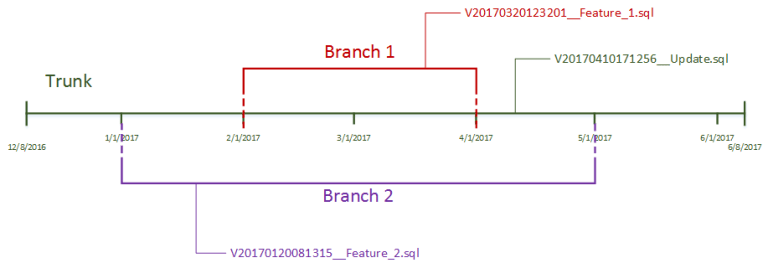
\includegraphics[width=0.95\textwidth]{./chapters/introduction/images/Branching-Flyway-Branch.png}
		\caption[Branching with Flyway - Source: \cite{Lukonin2017}]{Branching with Flyway}
		\label{fig:flyway_branching}
	\end{figure}

	
	
	\item Make sure to track all database changes\\
	Everyone should be able to see the latest change and history
	\item Store current schema version number in database\\
	To check weather the most recent version is deployed.
	\item Test changes\\
	If two migrations share the same name or you make a change that is influenced by another developer, it can quickly lead to a crash of the migration. So every migration or change on database artifacts has to be tested before and after every merge to the main branch to catch issues straight away.
	\item Each developer uses his own database and test databases resemble the production database.
\end{itemize}



\section{Available Tools}%
This section will provide an overview of available change management tools.
%The list of tools should include the available programming languages, price / availability
%and the main advantage over their competitors.

\begin{table}[h]
	\centering
	\begin{tabularx}{8cm}{X|c|l}
		Name & Language & Pricing \\ \hline
		Flyway & independent\\
		Liquibase & independent\\
		migrate & Go  \\
		Active Record Migrations & Ruby on Rails \\
		alembic & Python \\
		dbup & .NET \\
		Entity Framework Migrations & .NET \\
		Laravel Migrations & PHP \\
		\href{https://ollycope.com/software/yoyo/latest/}{Yoyo} &  \\
		\href{https://book.cakephp.org/phinx/0/en/migrations.html}{Phinx} &  \\
		\href{https://www.dbmaestro.com/for-devops}{DBmaestro} &  \\
		\href{https://docs.djangoproject.com/en/1.11/topics/migrations/}{Django} & Python \\
		\href{http://dbdeploy.com}{DBdeploy} & PHP \\
	\end{tabularx}
	\caption{Available migration tools - Based on \cite{}}
	\label{tab:migration_tools}
\end{table}


\todo{\url{https://www.quora.com/What-are-the-alternatives-to-LiquiBase}}


\section{Overview}%
This section will provide an overview of thesis.


\newpage